In recent years wide cloud adoption has caused huge momentum in adopting software architecture known as micro-services, as it is a native architecture for the cloud. This project will also adapt this architecture because part of the deployment is being done in the cloud, and a swarm of agents can also be simulated using this approach. Moreover, technologies such as kind and tilt made it easier to develop all services locally using the local Kubernetes cluster.

Micro-services are small autonomous services that cooperate with each other to create certain application logic\cite{building_microservices}. Usually, microservices are deployed as Linux containers and encapsulate logic for a single logical part of the solution. Those services are then communicating whit each other to build bigger, more complex systems.

\begin{figure}[H]
    \centering
    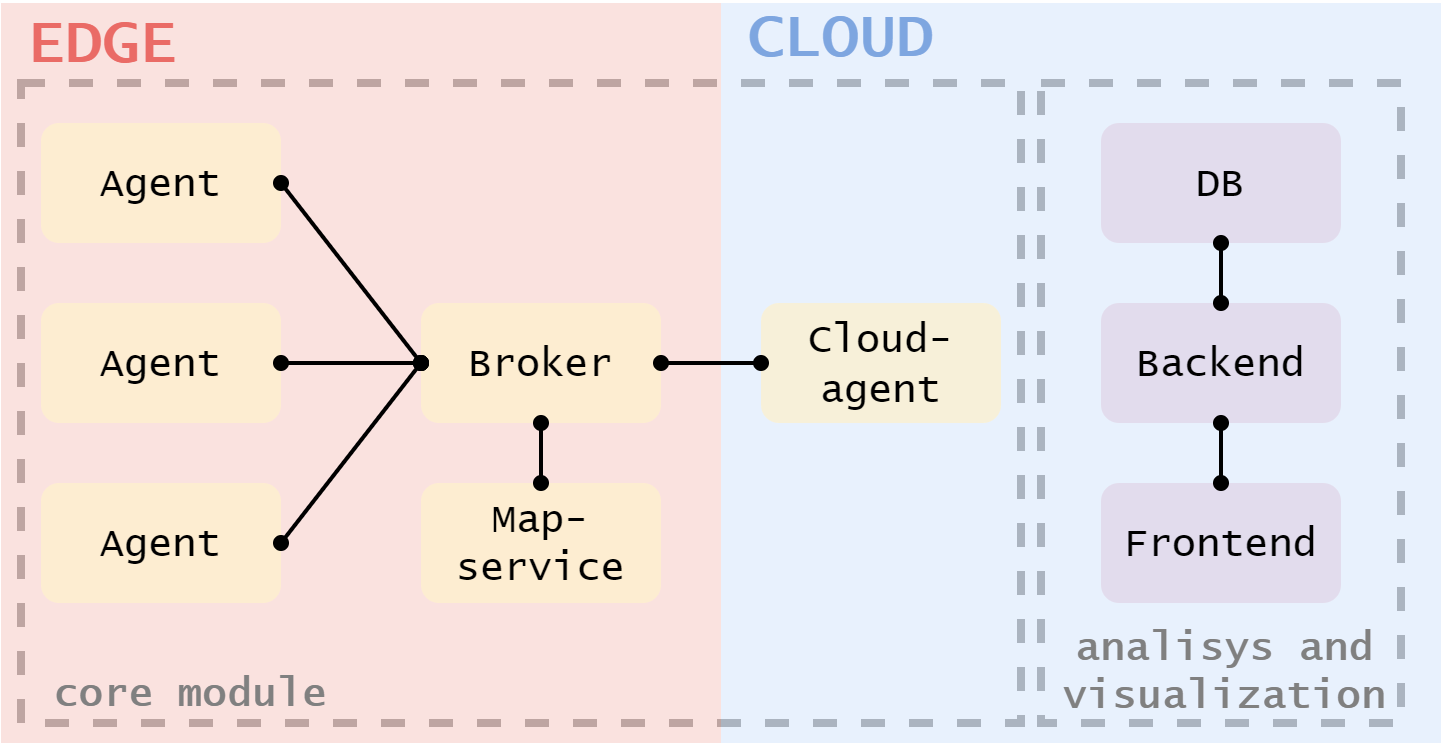
\includegraphics[width=\textwidth]{pictures/services.png}
    \caption{ Microservices system design }
    \label{fig:micro_services}
\end{figure}

\subsection{Agent}
The agent is a microservice which is implementing the logic of the entity which needs to plan a path.  It is meant to have limited resources to simulate a real-world scenario, and the number of its instances will vary.

When an agent is started, it doesn't belong to any swarm so it will start local discovery to find its peers. After peers are found, one of the agents has to be elected as a leader and therefore election algorithm will be initiated in one or multiple agents, so one of the agents will be elected to be a swarm leader. An agent will periodically poll his peers to check their liveness and this behavior will be referred to as a liveness check.

This entity contains also all algorithms meant for path planning as in a base case scenario, computation will take place in the agent to obtain the path.

\subsection{Cloud-agent}
The cloud-agent is a service that provides computational resources to offload the workload from agents. It is designed to have significantly more computing power than the agents, but it may be located in a different geographical location, which could result in latency issues when transmitting data back and forth.

In order to communicate with the agents, the cloud-agent uses the cloud-broker as a medium. The cloud-broker acts as an intermediary, enabling the cloud-agent and the agents to exchange messages and data.

The cloud-agent is deployed in the cloud and is intended to be used for performing computationally intensive tasks that would be too resource-intensive for the agents to handle on their own. By offloading these tasks to the cloud-agent, the agents are able to operate more efficiently and effectively.

\subsection{Broker}
This service plays a crucial role in the system, it is responsible for facilitating communication between various services. It is deployed both in the cloud and in local environments, and the two entities are connected by a bridge. The bridge serves as a single connection point between the cloud and the edge, allowing the two to communicate and exchange data.

Alternatively, the cloud and local services can also cross-subscribe to both brokers, allowing them to communicate directly with each other. The service uses a publish-subscribe (pub/sub) approach to handle and distribute messages between the different services.

The service acts as an intermediary, enabling services to exchange messages and data without the need for direct communication. This can help to reduce the complexity of the overall system and make it more scalable and resilient.

\subsection{Map-service}
This service is responsible for generating maps and spawning agents within them. When an agent is first created, it does not have any map assigned to it. The leader agent will trigger the generation of a new map by sending a message to the map-service. The map-service is responsible for creating the map and spawning the agent within it. Communication between the map-service and the agents is facilitated by the broker service. The broker service acts as an intermediary, enabling the map-service and the agents to exchange messages and data. It is through the broker service that the map-service sends the necessary information to the agents and receives requests and updates from them.

The map-service serves as a substitute for sensing for the agent, as it provides the robot with all the necessary information for determining its position on a global map. In addition to generating new maps, the map-service also stores pre-defined maps that can be adopted by the agent upon request.

It is possible for the map-service to spawn agents in places that are not reachable from the goal. This is a valid scenario as not all points on the map might be reachable. The map-service is a crucial component for enabling agents to navigate and interact with their environment.

\subsection{Backend}
This service is designed to gather data and facilitate communication with a core module service (such as an agent or map service) through a cloud broker. The service exposes endpoints through a REST API(appendix \ref{app:app_01}), which can be accessed by a frontend application. It also forwards requests to an MQTT broker.

In addition to interacting with other services, this service also receives data from various entities and stores it in a database. The backend of this service is deployed in the cloud, and the endpoints are accessible to end-users. It is equipped with a database for storing data. The database is attached to the service, which means that it is directly accessible and can be used for storing and retrieving data as needed. The service is designed to receive data from various entities, and it stores this data in the attached database for later use.

This service acts as an intermediary between the frontend, the core module service, and the MQTT broker, allowing them to communicate and exchange data. It is deployed in the cloud and connected to a cloud broker, which enables it to access resources and services hosted in the cloud.

\subsection{Frontend}
The frontend of this service is a graphical interface that is deployed as a web service. It is accessed by end users through a web browser and is used to trigger specific actions and perform raw data visualization.

The frontend is responsible for taking input from the end user and sending requests to the backend service through its API. It is also used for visualizing raw data, allowing the end user to view and analyze the data in various ways.

The frontend is deployed in the cloud and is exposed to end users over the internet. Its capabilities are further explained in the \hyperref[sec:0308]{visualization section} section of the documentation.

Frontend serves as the interface between the end user and the backend service, allowing the end user to interact with the service and access its functionality. It is an important component of the service, as it enables the end user to perform various actions and view raw data in an intuitive and user-friendly way.
